% Options for packages loaded elsewhere
\PassOptionsToPackage{unicode}{hyperref}
\PassOptionsToPackage{hyphens}{url}
\PassOptionsToPackage{dvipsnames,svgnames*,x11names*}{xcolor}
%
\documentclass[
  12pt,
]{article}
\usepackage{lmodern}
\usepackage{amssymb,amsmath}
\usepackage{ifxetex,ifluatex}
\ifnum 0\ifxetex 1\fi\ifluatex 1\fi=0 % if pdftex
  \usepackage[T1]{fontenc}
  \usepackage[utf8]{inputenc}
  \usepackage{textcomp} % provide euro and other symbols
\else % if luatex or xetex
  \usepackage{unicode-math}
  \defaultfontfeatures{Scale=MatchLowercase}
  \defaultfontfeatures[\rmfamily]{Ligatures=TeX,Scale=1}
\fi
% Use upquote if available, for straight quotes in verbatim environments
\IfFileExists{upquote.sty}{\usepackage{upquote}}{}
\IfFileExists{microtype.sty}{% use microtype if available
  \usepackage[]{microtype}
  \UseMicrotypeSet[protrusion]{basicmath} % disable protrusion for tt fonts
}{}
\makeatletter
\@ifundefined{KOMAClassName}{% if non-KOMA class
  \IfFileExists{parskip.sty}{%
    \usepackage{parskip}
  }{% else
    \setlength{\parindent}{0pt}
    \setlength{\parskip}{6pt plus 2pt minus 1pt}}
}{% if KOMA class
  \KOMAoptions{parskip=half}}
\makeatother
\usepackage{xcolor}
\IfFileExists{xurl.sty}{\usepackage{xurl}}{} % add URL line breaks if available
\IfFileExists{bookmark.sty}{\usepackage{bookmark}}{\usepackage{hyperref}}
\hypersetup{
  pdftitle={Statistical Learning Project},
  pdfauthor={1st Milestone},
  colorlinks=true,
  linkcolor=cyan,
  filecolor=Maroon,
  citecolor=Blue,
  urlcolor=magenta,
  pdfcreator={LaTeX via pandoc}}
\urlstyle{same} % disable monospaced font for URLs
\usepackage[margin=1.25cm]{geometry}
\usepackage{graphicx,grffile}
\makeatletter
\def\maxwidth{\ifdim\Gin@nat@width>\linewidth\linewidth\else\Gin@nat@width\fi}
\def\maxheight{\ifdim\Gin@nat@height>\textheight\textheight\else\Gin@nat@height\fi}
\makeatother
% Scale images if necessary, so that they will not overflow the page
% margins by default, and it is still possible to overwrite the defaults
% using explicit options in \includegraphics[width, height, ...]{}
\setkeys{Gin}{width=\maxwidth,height=\maxheight,keepaspectratio}
% Set default figure placement to htbp
\makeatletter
\def\fps@figure{htbp}
\makeatother
\setlength{\emergencystretch}{3em} % prevent overfull lines
\providecommand{\tightlist}{%
  \setlength{\itemsep}{0pt}\setlength{\parskip}{0pt}}
\setcounter{secnumdepth}{-\maxdimen} % remove section numbering
\usepackage{bbold}
\usepackage{amsmath}
\usepackage{hyperref}
\usepackage{mdframed, xcolor}
\usepackage{graphicx}
\mdfsetup{frametitlealignment=\center}
\usepackage{multirow}
\definecolor{shadecolor}{rgb}{0.89,0.8,1}
\newcommand{\Prob}{\mathbb{P}}
\newcommand{\Exp}{\mathbb{E}}
\newcommand{\Var}{\mathbb{V}\mathrm{ar}}
\newcommand{\Cov}{\mathbb{C}\mathrm{ov}}
\newcommand{\blue}{\textcolor{blue}}
\newcommand{\darkgreen}{\textcolor[rgb]{0,.5,0}}
\newcommand{\gray}{\textcolor[rgb]{.3,.3,.3}}
\newcommand{\blueA}{\textcolor[rgb]{0,.1,.4}}
\newcommand{\blueB}{\textcolor[rgb]{0,.3,.6}}
\newcommand{\blueC}{\textcolor[rgb]{0,.5,.8}}
\newcommand{\evidenzia}{\textcolor[rgb]{0,0,0}}
\newcommand{\nero}{\textcolor[rgb]{0,0,0}}
\newcommand{\darkyel}{\textcolor[rgb]{.4,.4,0}}
\newcommand{\darkred}{\textcolor[rgb]{.6,0,0}}
\newcommand{\blueDek}{\textcolor[rgb]{0.6000000, 0.7490196, 0.9019608}}
\newcommand{\purpLarry}{\textcolor[rgb]{0.6901961, 0.2431373, 0.4784314}}
\newcommand{\lightgray}{\textcolor[rgb]{.8,.8,.8}}
\newcommand{\bfun}{\left\{\begin{array}{ll}}
\newcommand{\efun}{\end{array}\right.}

\title{Statistical Learning Project}
\author{1st Milestone}
\date{Group 01 - Martina Betti, Stefano D'Arrigo, Leonardo Masci, Juan Mata}

\begin{document}
\maketitle

\hypertarget{research-title}{%
\subsection{Research Title}\label{research-title}}

Methods for improving Prof Brutti's run sessions

\begin{center}\rule{0.5\linewidth}{0.5pt}\end{center}

\hypertarget{abstract}{%
\subsection{Abstract}\label{abstract}}

The main aim of this project is to provide runners with a suitable
playlist for their day to day training, which can match the beat of each
runner's pace with the beat of their favourite songs. We will mainly
focus our attention on the use of interpretable machine learning
algorithms to predict the near future pace a runner will have. With
respect to the data collection task, we will be collecting our own
training session data through a variety of mobile phone applications and
potentially fitness tracking devices.

\begin{center}\rule{0.5\linewidth}{0.5pt}\end{center}

\hypertarget{project-update}{%
\subsection{Project Update}\label{project-update}}

We will enumerate the project updates below:

\begin{enumerate}
\item The most relevant update regarding the project is that we have recently decided not to use the \textit{steps} data provided by Google Fit. The rational behind this decision is that this information was only available for large intervals of time ($\sim$ 1 min), meaning we would lose granularity on the Arduino data if we were to merge them. Instead we will only use Google Fit data to extract information on Altitude and Distance, which is provided in a much more granular fashion (order of milliseconds as the Arduino data).
\item The merge between Arduino and Google fit will be performed by fixing the Arduino data timestamps, and imputing Google Data by performing a linear interpolation (linear interpolation will also be used to replace missing data in the Arduino measurements).
\item Among the difficulties we are facing in the data collection process we can highlight that for some of the users the Arduino App stops recording data abruptly after some random time. We are currently still trying to fix this by using other apps that might allow us to keep the phone active during our running session (e.g. Wakey). In the worst case scenario we will use the incomplete data. However, for two of the runners the Arduino App is able to collect data from start to end of the sessions.
\item We currently have around 10 running sessions for each user. The features that we are collecting are all those available in Arduino and the features Altitude and Distance from Google Fit.
\item All the raw data we have collected up to this point can be found under the following link: \href{https://drive.google.com/drive/u/1/folders/1mLCIF9zQHs7qVXGG03_Cj18c8y0vQie2}{Data Storage}.
\item A small sample of the already pre-processed and merged data sets can be found below. A larger sample of this data (already pre-processed) can also be found in the csv file delivered in the Milestone 2.
\end{enumerate}

Finally, we will also present some illustrative plots on the current
data:

\begin{figure}
\centering
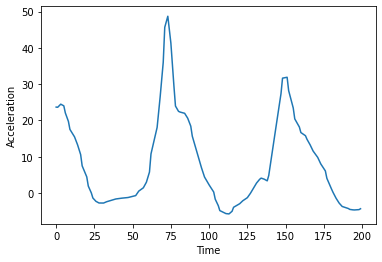
\includegraphics{200_points.png}
\caption{200 Data Points over the Y-Axis Acceleration}
\end{figure}

\begin{figure}
\centering
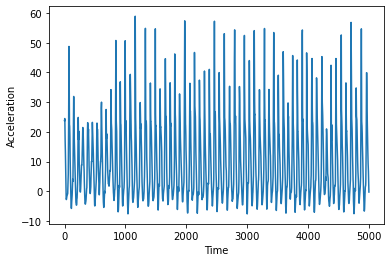
\includegraphics{Acc.png}
\caption{Y-Axis Acceleration over a longer time interval}
\end{figure}

\begin{figure}
\centering
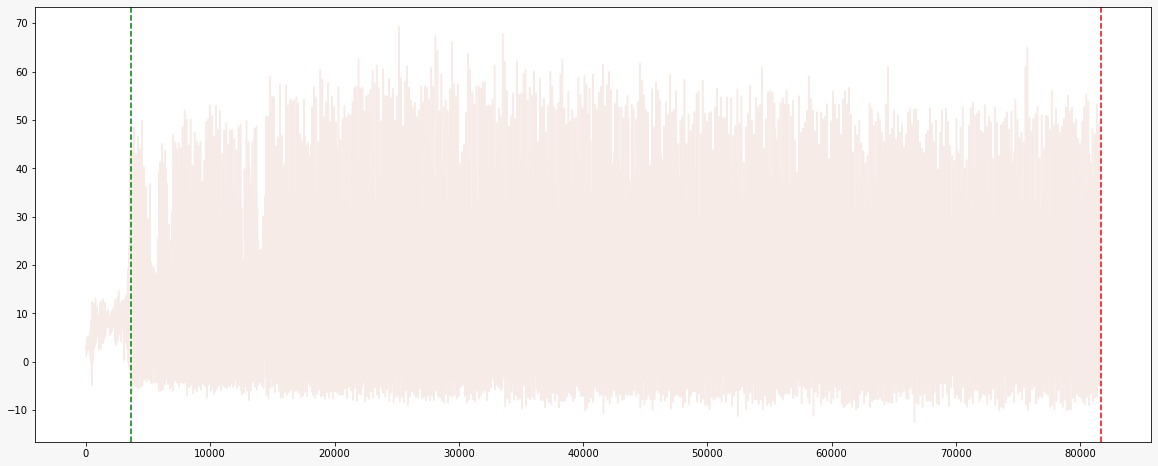
\includegraphics{StartStop.jpeg}
\caption{Start and End inference over a single run session}
\end{figure}

\begin{figure}
\centering
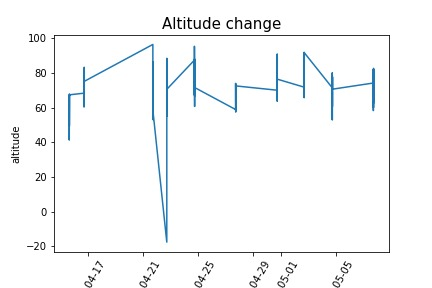
\includegraphics{Altitude.jpeg}
\caption{Altitude measurements over multiple running sessions}
\end{figure}

\begin{figure}
\centering
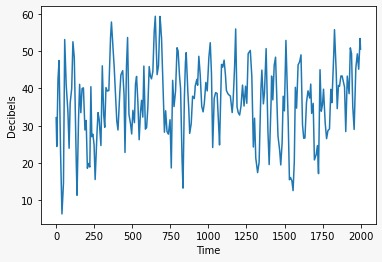
\includegraphics{Decibel.jpeg}
\caption{Decibel Timeseries for 2000 time stamps}
\end{figure}

\newpage

\begin{center}\rule{0.5\linewidth}{0.5pt}\end{center}

\hypertarget{updated-project-timeline}{%
\subsection{Updated Project Timeline}\label{updated-project-timeline}}

\begin{figure}
\centering
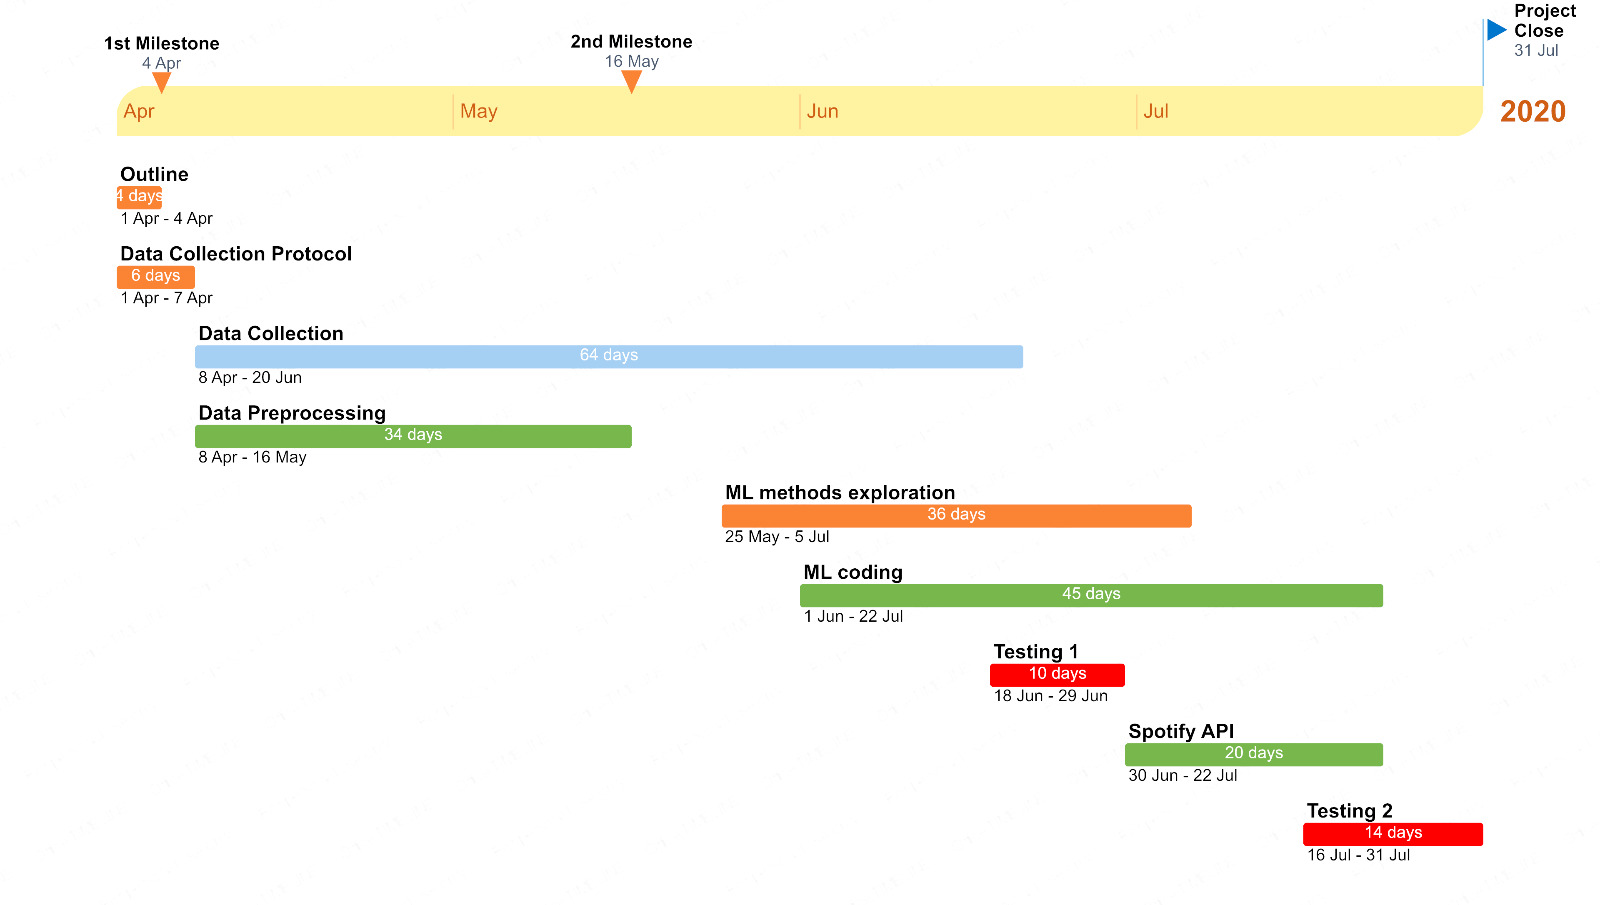
\includegraphics{Timeline.jpg}
\caption{Timeline}
\end{figure}

The data pre-processing phase of the project is already complete, and we
foresee to start working on the modeling part after the 25 of May. The
next sections of this report have not changed since the last Milestone.

\begin{center}\rule{0.5\linewidth}{0.5pt}\end{center}

\hypertarget{main-research-aim-framework}{%
\subsection{Main research aim \&
framework}\label{main-research-aim-framework}}

The main aim of this project is to provide runners with a suitable
playlist for their day to day training. There are a wide range of papers
that have shown that music has a very large impact on the performance of
a runner ({[}3{]}). There are however fewer papers and apps that
actively try to use music to improve the runner's pace/cadence. Between
these few apps and papers we can highlight: {[}4{]} and
\href{https://run.weav.io/}{Weav Run}. The main goal can therefore be
decomposed into two smaller prediction goals:

\begin{itemize}
\item Predict the running pace/cadence of each individual based on their past training sessions and some additional features (e.g. audio, heart beat, linear acceleration, steps, altitude, etc.).
\item Play songs that can match the current and possibly future cadence of the runner so that the runner can stay motivated at all times.
\end{itemize}

Secondary goals that can also be considered depending on the time and
intermediate issues that may appear on the way:

\begin{itemize}
\item Can we also apply this to other activities (cycling, walking, boxing, etc.)?
\item Besides the song’s beat, can we also see what type of music suits runners best and therefore recommend other songs that are not in the playlist to the user?
\end{itemize}

\begin{center}\rule{0.5\linewidth}{0.5pt}\end{center}

\hypertarget{iml-papers-you-like-at-this-point-review}{%
\subsection{IML paper(s) you like (at this point!)
(review)}\label{iml-papers-you-like-at-this-point-review}}

According to the article {[}10{]}, there are three levels of
interpretability:

\begin{itemize}
\item Statistical interpretability, which aims to uncover statistical associations to assess how seeing x would change our belief in y
\item Causal interventional interpretability, which is designed to define how a change in x could affect y
\item Counterfactual interpretability, which intends to explain why x affects y.
\end{itemize}

Speaking in terms of ``final goal'', our work will mainly be focused on
the statistical level. However, since we want to keep our model as
simple and understandable as possible, it will be necessary to
investigate which of the features (x) are actually relevant for the
prediction (y) and which are not.

Despite our final goal being to look for interpretability at statistical
level, we also found some of the papers on counterfactual level
interesting (also known as post-hoc interpretability as defined in
{[}5{]}): The paper {[}8{]} uncovers more complex models by finding the
nearest counterfactual explanation by minimizing the following
expression relying on SMT techniques:

\begin{align}
\hat{\boldsymbol{x}}^* \in \operatorname*{argmin}_{\boldsymbol{x} \in CF_f(\hat{\boldsymbol{x}})} d(\boldsymbol{x}, \hat{\boldsymbol{x}})
\end{align}

where \(CF_f(\hat{\boldsymbol{x}})\) contains all the inputs x for which
the model \(f\) returns a prediction different from
\(f(\hat{\boldsymbol{x}})\) (so basically we are fixing
\(\hat{\boldsymbol{x}}\) and also \(f\), and we look for all of the
input feature vectors that live in \(X\) such that the predictions are
different) and \(d\) is any appropriate distance measure between the
feature vectors \(\hat{\boldsymbol{x}}\) and \(\boldsymbol{x}\).

As a last remark though, and quoting from the paper of Rudin {[}11{]} we
will initially try to build our machine learning model in such a way
that it is as interpretable as possible, without needing any additional
explainable model that interprets the results.

\begin{center}\rule{0.5\linewidth}{0.5pt}\end{center}

\hypertarget{data-sources}{%
\subsection{Data source(s)}\label{data-sources}}

We aim to make use of the
\href{https://play.google.com/store/apps/details?id=cc.arduino.sciencejournal\&hl=en}{Arduino
Science Journal app}, running on four different models of Android
smartphones in order to collect the accelerometer and other sensors'
measurements recorded during a running session. Furthermore, we plan to
exploit the functionalities of fitness and sports apps; at this stage of
the project development, we selected the
\href{https://play.google.com/store/apps/details?id=com.google.android.apps.fitness\&hl=en}{Google
Fit} app, which provides information regarding the steps' count, the
distance, the speed, the altitude and other derived variables in a
structured file format. Nevertheless, additional software may be
required to expand the feature set. Finally, we reckon that just our
smartphones and, maybe, a couple of wearable devices will be needed. For
the music recommender module, we will rely on the Spotify REST API and
other web services,
e.g.~\href{https://www.cs.ubc.ca/~davet/music/index.html}{Music
Database, University of British Columbia}.

\begin{center}\rule{0.5\linewidth}{0.5pt}\end{center}

\hypertarget{data-collection}{%
\subsection{Data collection}\label{data-collection}}

The data will be recorded during at least 20 running sessions throughout
the entire project development (see the project schedule in the section
below); each session will be carried out individually for about 30
minutes, making use of the aforementioned software and hardware tools;
at the end of the collection, we aim to have four individual data sets -
one for each group member -, that will be handled independently from
each other. These raw measurements are expected to require order of
hundreds of Megabytes or few Gigabytes storage. Dealing with general
purpose sensors and commercial applications and since the records will
be captured outdoor, in potentially unpredictable environments, noise
removal will be particularly challenging.

\begin{center}\rule{0.5\linewidth}{0.5pt}\end{center}

\hypertarget{model-methods}{%
\subsection{Model \& Methods}\label{model-methods}}

We would like to implement some multivariate time series models, as we
feel that our data will be best analysed when interpreted as a time
series. Each run would be added on to the global time series, so that in
the end a model would be created for each individual runner.

Given that we will work with time series data, before starting to do any
predictions we will first need to do some additional data exploration
and pre-processing:

\begin{itemize}
\item \textbf{Seasonal variations:} Which in this case would take the form of a pattern identifiable within each single run (for example, a slower start and end of the run, compared to the pace in the middle of it)
\item \textbf{Secular trend:} Which would identify any improvement of performance of the runner over time
\item \textbf{Irregular variations and cyclical fluctuations:} Which are to be ignored
\item \textbf{Time series smoothing:} Required given the high volatility of time series data. Some techniques that we will be inspecting are moving average smoothing, exponential smoothing, etc.
\end{itemize}

Once the time series have been processed properly, some models that will
initially be investigated are the following:

\paragraph{ARIMA}

The ARIMA is a class of models that `explains' a given time series based
on its own past values, so that equation can be used to forecast future
values. ARIMA results from the combination of three procedures:
Autoregression, integration and Moving Averages. It can be represented
by the equation:

\begin{align}
I^i_t = \delta + \sum_{i=1}^p \phi_i I_{t-1}^{'} + \sum_{i=1}^q \theta_i e_{t-1}+e_t
\end{align}

where \emph{p} is the order of the AR term, \emph{q} is the order of the
MA terms and \emph{I} depends on the number of differentiating required
to make the time series stationary.

ARIMA can model homogeneous non-stationary series, like time series with
a non-explosive trend, however if the data presents seasonality patterns
the series may also have autocorrelation for a seasonal station s. In
this context we can use the seasonal ARIMA models, also known as SARIMA.

\paragraph{ARIMAX}

The ARIMAX model is an extension of the previous one, in the sense that
it adds an exogenous variable (so an external one) to help in measuring
the endogenous variable of interest. For this reason, the related
formula is also very similar to the one of ARIMA: only X and its
coefficient \(\beta\) have to be added to the previous equation

\paragraph{VAR}

The VAR (Vector Autoregression) model is another statistical model and
it has proven to be particularly suitable for analyzing multivariate
time series that influence each other. Aiming to describe the evolution
of \(k\) variables over time, its power lies on the inclusion of
\emph{lags}, i.e.~it takes into account the values of the variables in
the previous time period. Depending on the number of \emph{lags}, say
\(p\), the \(p\)-th order VAR model is expressed as:

\[
y_t = c + \sum_{i=1}^{p} A_i y_{t-i} + e_t
\]

having \(y_{t-i}\) the \(i\)-th lag, \(c\) a vector of constants,
\(A_i\) a time-invariant matrix and \(e_t\) a vector of errors related
to the current \(t\) time series.

In order to find the best performing model between these for each
individual, we will rely on some sample splitting methods in order to
make our model selection more robust on new data (e.g.~k-fold CV,
LOOCV).

There has been a lot of research in recent years in the field of
interpretable machine learning for multivariate time series forecasting
since most state-of-the-art models involved in this activity are deep
learning models which ultimately act as black boxes. Some of the papers
that try to tackle these issues are {[}2{]}, {[}6{]}. If we are not able
to get satisfactory results with more interpretable models and have to
leverage on black box models, interpreting them using the techniques
described in the previous papers could be a good idea.

\begin{center}\rule{0.5\linewidth}{0.5pt}\end{center}

\hypertarget{softwarehardware-toolkit}{%
\subsection{Software/Hardware Toolkit}\label{softwarehardware-toolkit}}

We are going to use pandas for any preprocessing that may be needed, and
proceed with python for the actual coding. Based on the models we will
employ, we are going to work with their appropriate packages.

For the music part of it, we are going to work with
\href{https://spotipy.readthedocs.io/en/2.17.1/}{Spotipy}, a Python
library for the Spotify Web API. Finally, for the data collection, we
are going to make use of the above mentioned mobile apps.

\begin{center}\rule{0.5\linewidth}{0.5pt}\end{center}

\hypertarget{references}{%
\subsection{References}\label{references}}

\begin{itemize}
\tightlist
\item
  \protect\hypertarget{1}{}{{[}1{]}} Bäärnhielm, A. (2017).
  \emph{Multiple time-series forecasting on mobile network data using an
  RNN-RBM model}.
\item
  \protect\hypertarget{2}{}{{[}2{]}} Barbieri, S., Kemp, J.,
  Perez-Concha, O. et al.~\emph{Benchmarking Deep Learning Architectures
  for Predicting Readmission to the ICU and Describing
  Patients-at-Risk.} Sci Rep 10, 1111 (2020).
  \url{https://doi.org/10.1038/s41598-020-58053-z}
\item
  \protect\hypertarget{3}{}{{[}3{]}} Bly, Kristopher, \emph{The effect
  of music playlist tempo on self-paced running, mood, and attentional
  focus tendencies} (2013), Ithaca College Theses. 12.
  \url{https://digitalcommons.ithaca.edu/ic_theses/12}
\item
  \protect\hypertarget{4}{}{{[}4{]}} Buhmann J, Moens B, Van Dyck E,
  Dotov D, Leman M (2018) \emph{Optimizing beat synchronized running to
  music}. PLoS ONE 13(12): e0208702.
  \url{https://doi.org/10.1371/journal.pone.0208702}
\item
  \protect\hypertarget{5}{}{{[}5{]}} Laugel, Thibault \& Lesot, Marie \&
  Marsala, Christophe \& Renard, Xavier \& Detyniecki, Marcin. (2017).
  \emph{Inverse Classification for Comparison-based Interpretability in
  Machine Learning}.
\item
  \protect\hypertarget{6}{}{{[}6{]}} L. Pantiskas, K. Verstoep and H.
  Bal, \emph{``Interpretable Multivariate Time Series Forecasting with
  Temporal Attention Convolutional Neural Networks,''} 2020 IEEE
  Symposium Series on Computational Intelligence (SSCI), Canberra, ACT,
  Australia, 2020, pp.~1687-1694, doi: 10.1109/SSCI47803.2020.9308570.
\item
  \protect\hypertarget{7}{}{{[}7{]}} Katardjiev, N. (2018).
  \emph{High-variance multivariate time series forecasting using machine
  learning (Dissertation)}. Retrieved from
  \url{http://urn.kb.se/resolve?urn=urn:nbn:se:uu:diva-353827}
\item
  \protect\hypertarget{8}{}{{[}8{]}} Karimi, A., Barthe, G., Balle, B.
  \& Valera, I.. (2020). \emph{Model-Agnostic Counterfactual
  Explanations for Consequential Decisions. Proceedings of the Twenty
  Third International Conference on Artificial Intelligence and
  Statistics}, in \emph{Proceedings of Machine Learning Research}
  108:895-905 Available from
  \url{http://proceedings.mlr.press/v108/karimi20a.html}
\item
  \protect\hypertarget{9}{}{{[}9{]}} Parmezan, Antonio. (2019).
  \emph{Re: What are the best machine learning algorithms for time
  series forecasting}?. Retrieved from:
  \url{https://www.researchgate.net/post/What-are-the-best-machine-learning-algorithms-for-time-series-forecasting/5d7e74010f95f1bedb676868/citation/download}.
\item
  \protect\hypertarget{10}{}{{[}10{]}} Raha Moraffah, Mansooreh Karami,
  Ruocheng Guo, Adrienne Raglin, and Huan Liu. 2020. \emph{Causal
  Interpretability for Machine Learning - Problems, Methods and
  Evaluation}. SIGKDD Explor. Newsl. 22, 1 (June 2020), 18--33.
  \url{DOI:https://doi.org/10.1145/3400051.3400058}
\item
  \protect\hypertarget{11}{}{{[}11{]}} Rudin, C. \emph{Stop explaining
  black box machine learning models for high stakes decisions and use
  interpretable models instead}. Nat Mach Intell 1, 206--215 (2019).
  \url{https://doi.org/10.1038/s42256-019-0048-x}
\item
  \protect\hypertarget{12}{}{{[}12{]}} Wagner, N., Michalewicz, Z.,
  Schellenberg, S., Chiriac, C. and Mohais, A. (2011),
  \emph{``Intelligent techniques for forecasting multiple time series in
  real‐world systems''}, International Journal of Intelligent Computing
  and Cybernetics, Vol. 4 No.~3, pp.~284-310.
  \url{https://doi.org/10.1108/17563781111159996}
\end{itemize}

\begin{center}\rule{0.5\linewidth}{0.5pt}\end{center}

\end{document}
